\chapter{Křivky v praxi}
Pokud se pozorně porozhlédnete kolem sebe, jistě někde uvidíte kružnici nebo kruh, ať už je to okraj hrnečku, prstýnek na ruce
nebo kruhová značka. \\
Kruhová okna (rozety) pak můžeme vidět na gotických chrámech. \\
\begin{figure}[H]
	\centering
	\includegraphics[height=0.3\textheight]{rozeta.jpg}
	\caption{Rozeta v kostele svatého Matyáše v Richmondu v Anglii}
	\label{overflow}
\end{figure}
Velmi často se setkáme také s elipsou. Stačí vzít válcovou skleničku s vodou (ne úplně plnou) a tu trochu naklonit.
Povrch vodní hladiny je ohraničen elipsou. Nebo ukrojte našikmo válcovou šišku salámu. Elipsu můžeme vidět i v architektuře,
zejména v barokní architektuře (půdorysy staveb aj.). \\
Kovová vrata u metra Malostranská v Praze jsou sestaveny z mnoha nejrůznějších elips. \\
Svítí-li vhodně Slunce, jsou stíny na zdech zase elipsy (jiné než na vratech). \\
\begin{figure}[H]
	\centering
	\includegraphics[height=0.3\textheight]{malostranska.jpg}
	\caption{Elipsy na vratech u stanice metra Malostranská v Praze}
	\label{overflow}
\end{figure}
V architektuře najdeme také části parabol, jsou to často mostní oblouky. \\
\begin{figure}[H]
	\centering
	\includegraphics[height=0.3\textheight]{bachyne.jpg}
	\caption{Mostní oblouk v Bechyni tvořen částí paraboly}
	\label{overflow}
\end{figure}
U administrativní budovy v Českých Budějovicích je využita parabola pro ohraničení oken. Válcová věž
je zastřešena šikmou střechou, hraniční mnohoúhelník je náhradou elipsy. \\
\begin{figure}[H]
	\centering
	\includegraphics[height=0.3\textheight]{cb.jpg}
	\caption{Administrativní budova v Českých Budějovicích}
	\label{overflow}
\end{figure}
Co se týče hyperboly, můžete mít pocit, že tu hned neuvidíme. Ale vezměte si lampu se stínítkem
zakončeným kružnicí v rovině rovnoběžné s podlahou. Lampu postavte blízko zdi. Hranice mezi stínem
a světlem je část hyperboly.
\begin{figure}[H]
	\centering
	\includegraphics[height=0.3\textheight]{lampa.jpg}
	\caption{Hranice mezi stínem a světlem je část hyperboly}
	\label{overflow}
\end{figure}
Jistě dokážete naklonit lampu tak, aby hranicí byla elipsa nebo část paraboly. \\[5pt]
Co se týče prostorových křivek, nejčastěji uvidíme šroubovici. Bývá to zábradlí točitých schodišť.
Na obrázcích jsou schodiště z Lorettské kaple a z Vatikánského muzea.
\begin{figure}[H]
	\centering
	\includegraphics[height=0.3\textheight]{schodiste.jpg}
	\caption{Točité schodiště v Lorettské kapli v Santa Fe v Novém Mexiku}
	\label{overflow}
\end{figure}
\begin{figure}[H]
	\centering
	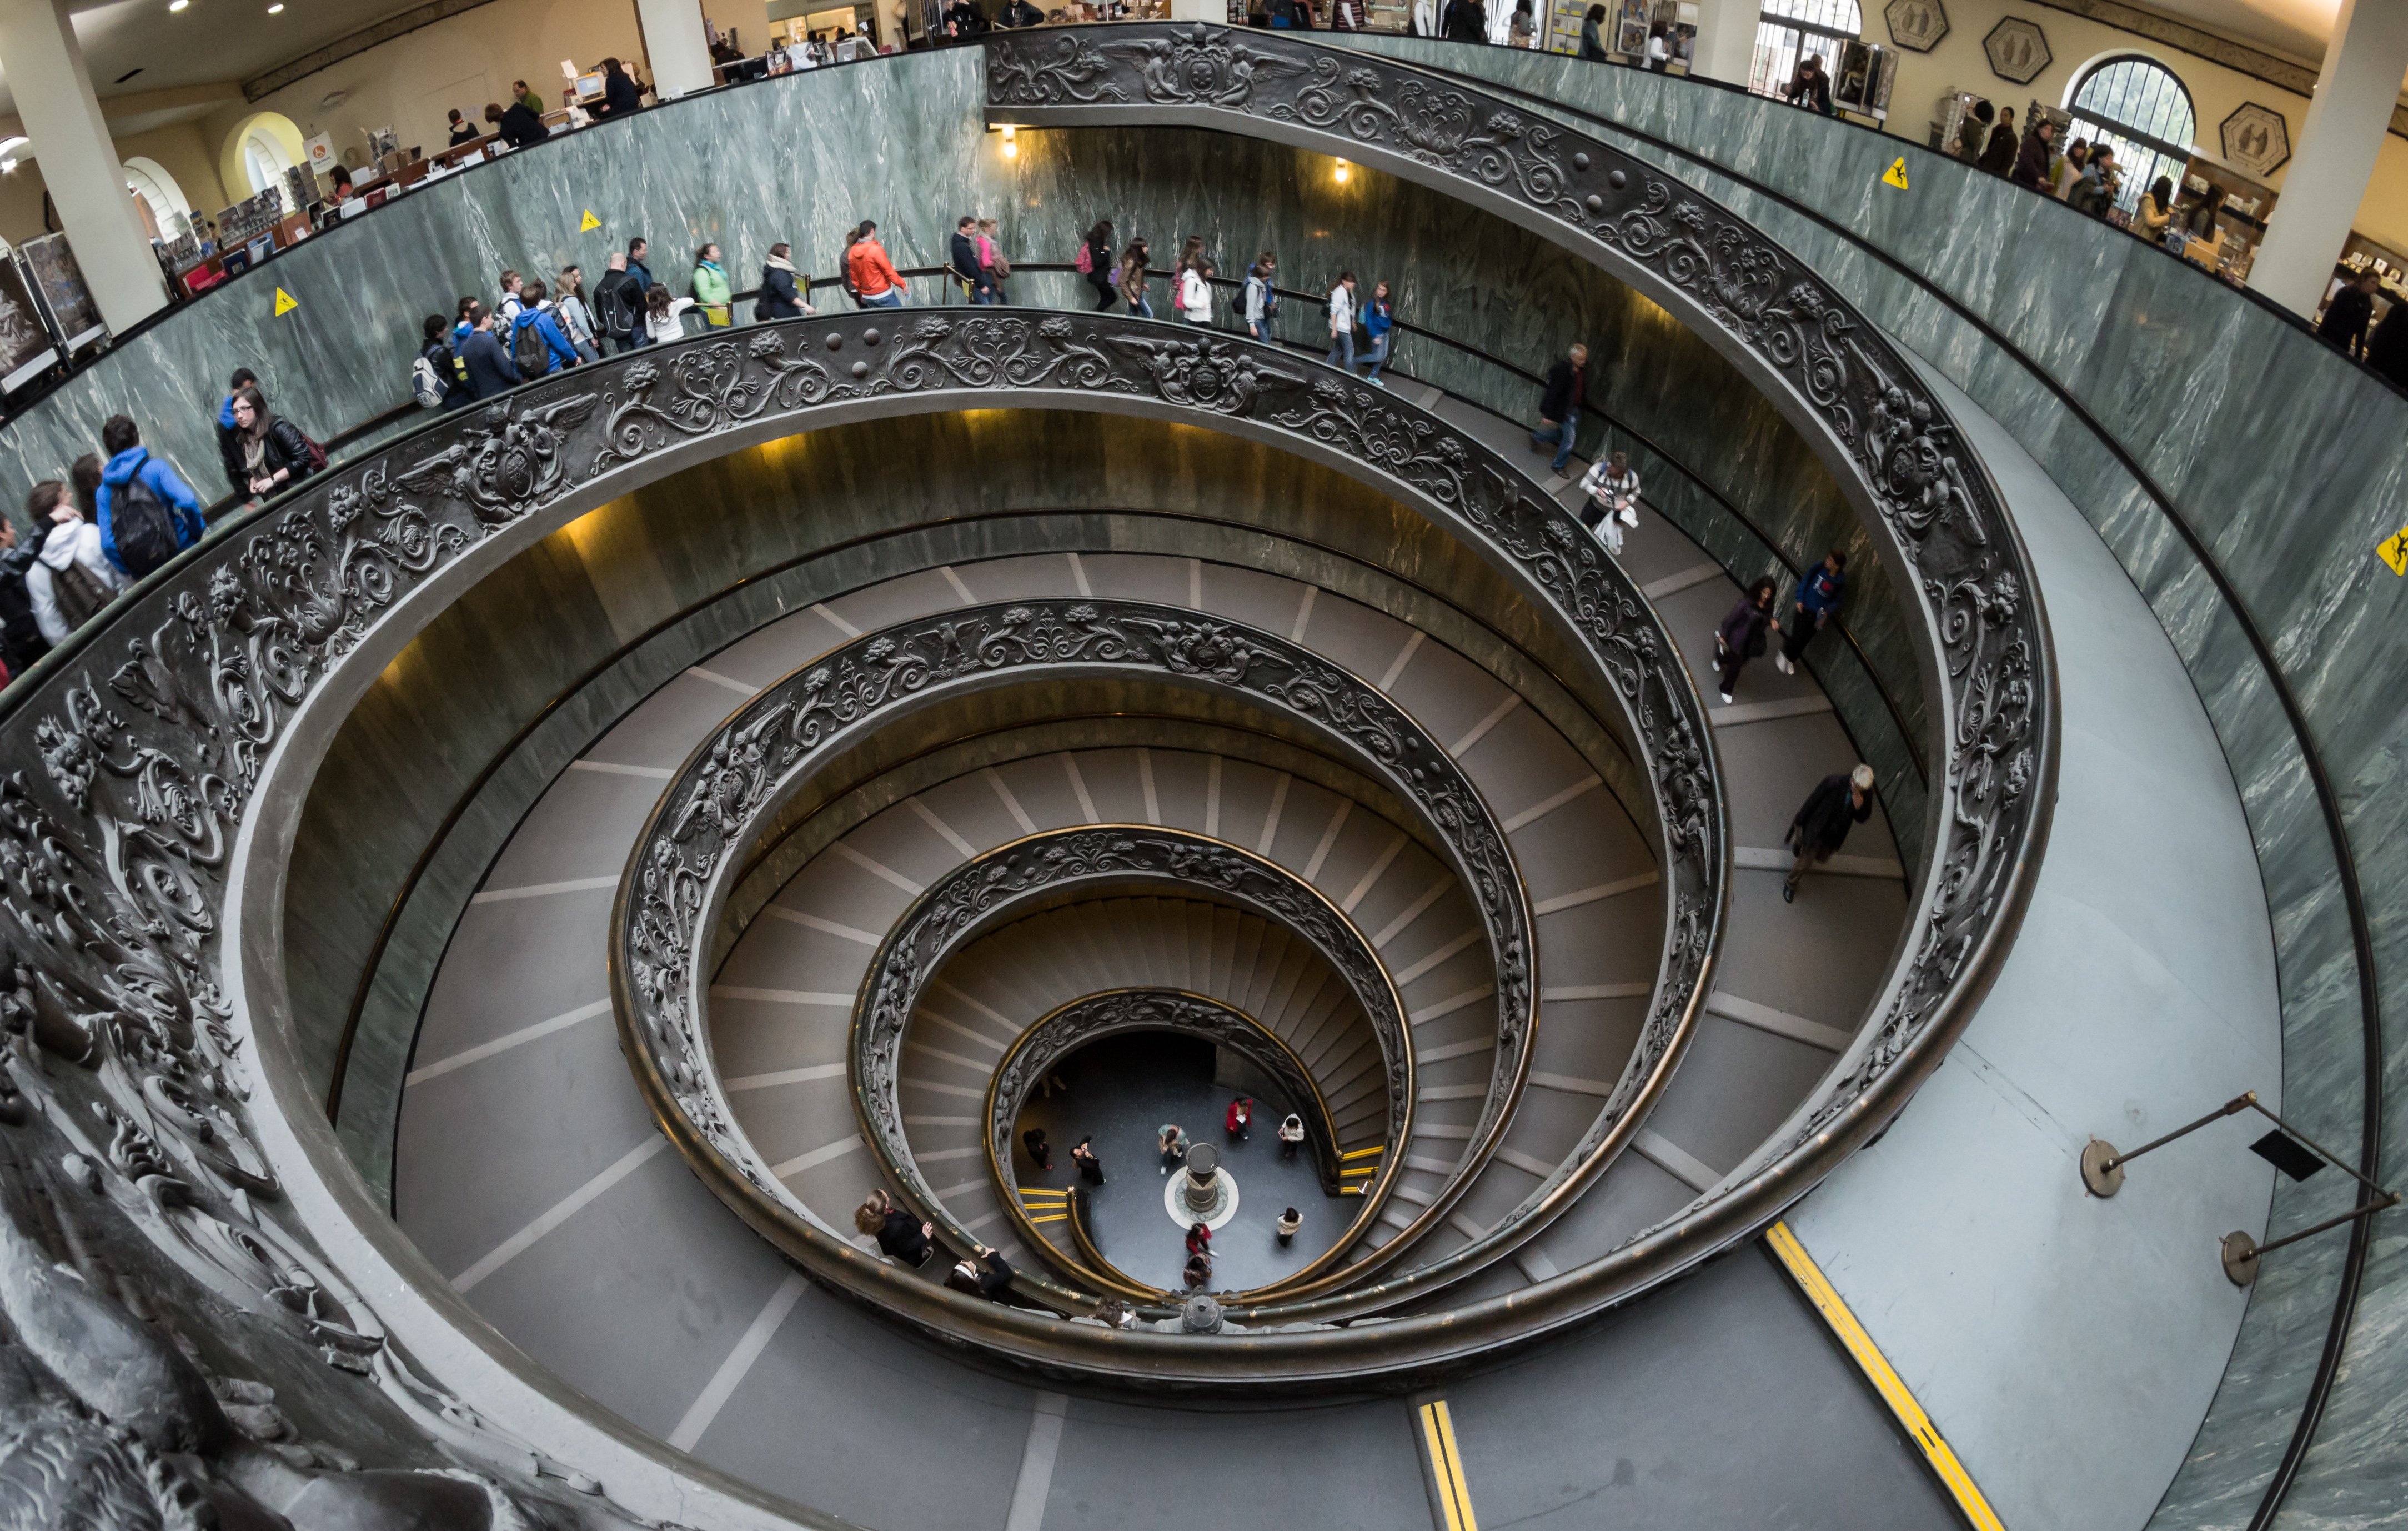
\includegraphics[height=0.3\textheight]{schodiste2.jpg}
	\caption{Točité schodiště tvořené dvoušroubovicí ve Vatikánském muzeu}
	\label{overflow}
\end{figure}
Jistě si ještě vzpomenete na šrouby, vývrtky aj. V neposlední řadě si připomeneme molekulu \textit{DNA}
(deoxyribonukleové kyseliny), ačkoliv tu vidět pouhým okem nemůžeme vzhledem k jejím rozměrům. \textit{DNA}
má tvar pravotočivé dvoušroubovice (ale může být i levotočivá). Dvě šroubovice mají společnou osu a stejnou výšku
závitu \textit{v}, jen jsou vzájemně posunuty (posunutí ve směru společné osy). Poznamenejme, že existují i jiné
způsoby uspořádání.
\begin{figure}[H]
	\centering
	\includegraphics[height=0.3\textheight]{dna.png}
	\caption{DNA má tvar pravotočivé šroubovice}
	\label{overflow}
\end{figure}
\begin{figure}[H]
	\centering
	\includegraphics[height=0.3\textheight]{dna2.png}
	\caption{Další struktury DNA}
	\label{overflow}
\end{figure}